\section{Problem Statement}
\label{sec:problemStatement}

% \begin{figure}[t]
%     \centering
%     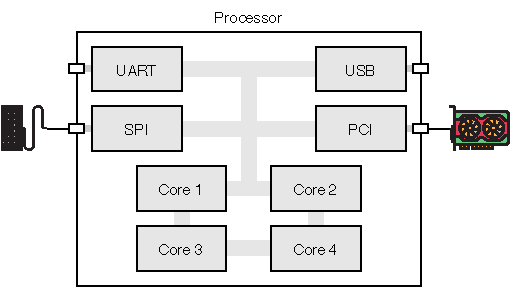
\includegraphics[width=0.9\linewidth]{images/cpu_bus_peripheral-Page-1.pdf}
%     \caption{A typical bus architecture of a platform where the cores are connected to on-chip bus controllers such as PCI and USB, wich are in turn connected to external \sphw devices. E.g, the GPU and the keyboard is connected via the PCI-E controller and SPI bus respectively.}
%     \label{fig:bus}
% \end{figure}


Modern platforms are composed of complex heterogeneous \sphw, from simple sensors that measure temperature or humidity to complex accelerators for machine learning. All these components are connected to the CPU over buses (e.g., PCI, USB, etc.). % as depicted in Figure~\ref{fig:bus}.
Many modern applications are critically dependent on such \sphw, and often they handle sensitive data, e.g., patient records for machine learning. Thus, these \sphw{}s' authenticity and integrity are critical, and the data they handle must remain confidential. 
% We list three such applications in the following:

% \paragraph{Application 1: Isolated execution on accelerators} 
% Many science fields require a vast amount of computation power, which a general-purpose processor can no longer provide. In recent times, specialized hardware which is very efficient for one specific problem is used in the form of accelerators, e.g., machine learning accelerators in the cloud. Such applications often handle sensitive data such as patient records and require isolation from the OS and other applications running on the same GPU. %Besides, these accelerators might need to be connected to live measurements such as a camera and process the inputs in real-time.

% \paragraph{Application 2: Trusted sensor readings}
% Safety-critical industrial and medical devices rely on measurements of critical sensors. E.g., a pressure sensor provides data to the industrial controller, who decides when to open a safety valve.
    
% \paragraph{Application 3: Trusted path for IO devices} A user uses her IO devices (keyboard, mouse, display, etc.) to interact with an online banking application running on her device. The user wants to verify that the banking application is exclusively accessing her IO devices. In this case, the user wants to harden her system against a potentially compromised software stack.

%\moritz{Should we go more into the direction of remote systems vs hardening measures?}

Applications that handle sensitive data and use a \sphw device can be deployed securely with one of the following three existing approaches: 1) designing a fully dedicated system, or 2) renting a dedicated virtual machine and placing trust in the hypervisor, or 3) relying on the OS. None of these approaches to be satisfactory due to lack of generality, cost, and the need to trust codebases with millions of lines of code~\cite{torvalds2020linux,barham2003xen}. Existing TEEs such as Intel SGX, RISC-V Keystone, ARM TrustZone, etc., provide security guarantees only to the applications running on the CPU cores leaving \sphw unprotected. Moreover, SGX and Keystone enclaves rely on the untrusted OS to communicate with \sphw. On the other hand, ARM TrustZone provides isolated communication between the enclaves and components such as a touchscreen, fingerprint sensor, but requires trusting the entire secure OS, including device drivers not used by the enclave.  %Graviton~\cite{volos2018graviton} proposes isolated enclaves on the GPU that communicate securely with the SGX enclaves. But its geared to a GPU can cannot be extended to generic \sphw.


\subsection{Attacker Model}
\label{sec:problemStatement:attackerModel}

The attacker model is tightly coupled with the type of \sphw. We separate the \sphw into two main classes due to their distinct effect on the attacker model: 
%\sphw that explicitly interact with their physical environment and those that do not. Intuitively, sensors interact with their environment by taking measurements. Accelerators, however, do not explicitly interact with the real-world. The \sphw classes and their respective attacker models are described in the following:

\begin{enumerate}
\item \emph{\Sphw with physical interaction:}
\Sphw that interact with their environment range from input-only, such as input peripherals (e.g., mouse, keyboard) and sensors (e.g., temperature sensor) to output-only devices (e.g., monitor) and combined IO devices (e.g., touchscreen). For any such device, a local physical adversary can manipulate the environment and thus the input (and potentially the output). E.g., a physical adversary can point a laser at a light sensor, thus changing the sensor's reading but not the room's overall light intensity. Hence, any \sphw that interacts with its physical environment cannot tolerate a physical adversary.

\item \emph{\Sphw without physical interaction:}
There are \sphw units that do not explicitly interact with their environment. They draw power and produce heat, but their input and output are not related to the environment. GPUs and other accelerators are the prime examples of this class of \sphw, for whom a local physical adversary can be tolerated. 
\end{enumerate}

In this paper, we assume a remote attacker that remotely controls the entire software stack, including the OS and hypervisor. While the remote attacker model is a weaker assumption compared to the local physical one considered in the existing TEEs, the former covers a wide class of \sphw (e.g., \sphw with physical interaction) that cannot tolerate physical attackers. Hence, the attacker cannot access the platform of the \sphw physically or hot-swap a device. Note that the untrusted OS is still in charge of managing \sphw devices, and thus is able to remap the devices or send a reset or power-off signal.
We assume that the CPU firmware is trusted. Similar to existing TEE proposals, side channel attacks remain out of scope~\cite{costan2016intel} in our adversary model. However, we will discuss the implications of our proposal on existing side channel attacks and defenses in \Cref{sec:securityAnalysis}. Finally, we consider denial-of-service attacks to be out of scope in this paper. 


\subsection{Challenges}
\label{sec:problemStatement:challenges}
%\moritz{Needs to be adapted to intro. (and better formulated).}
As mentioned above, several approaches could be pursued to integrate \sphw into a TEE. Among them, we investigate approaches that reuse components of existing systems as much as possible, both in terms of software and in terms of hardware.  
%A modern platform's computation capability is distributed over \sphw units with the CPU acting as a coordinator. For computation tasks on sensitive data, the data's integrity and confidentiality is crucial in all devices. The TCB should remain configurable and only include the application running on the CPU and the driver and the firmware of the \sphw device it is accessing. 
%In this paper, we address this by investigating enclaves that span an entire platform, which we call \emph{\nameenclave{}s}. In addition, the hardware and software TCB of a \nameenclave{} should be configurable and thus adhere to the principle of least privilege. 
%In this paper, we investigate enclaves that span an entire platform as distributed enclaves constructed from individual and asynchronous enclaves.
This approach leaves the OS in a supervisor role, liaising between the isolated environments and \sphw, similar to memory in traditional TEEs (c.f. Section~\ref{sec:background}). But, this decision leaves leeway for privileged adversaries to break the system's isolation. We therefore need to consider both existing threats to traditional TEEs and emerging threats due to the nature of a reconfigurable hardware TCB. 
% As analyzed in CPU-centric TEEs~\cite{checkoway2013iago}, this approach leaves leeway for privileged attackers to break the system's isolation. We therefore need to take into account both these threats and the ones that emerge due to the nature of a reconfigurable hardware TCB. 
We analyze these in more detail in the next three paragraphs.

% Extending the TEEs to the entire platform is non-trivial and comes with several challenges, especially in the application scenarios that we discussed previously in Section~\ref{sec:problemStatement}. There exists a few proposals of TEEs that consider \sphw, such as solutions~\cite{VButton,SeCloak} based on ARM TrustZone. However, they require all the \sphw present in the platform in the TCB. We consider a \name to be a combination of multiple TEEs on individual components, e.g., a TEE on the CPU~\cite{sgx,keystone} and one on the GPU~\cite{volos2018graviton}. A \name{} should provide similar guarantees as traditional TEEs and eventually pave the way for secure computation on an entire platform.

\myparagraph{Secure communication}
Traditionally, the OS or the hypervisor act as the bridge between applications and \sphw. They are responsible to set-up these communication links properly, and can not only observe the data exchanged between different components, but also tamper with it.
%However, OS and hypervisors are usually large codebases with hundreds of lingering vulnerabilities~\cite{checkoway2013iago,suzaki2011memory}
As they are not trusted in our attacker model, we need to ensure that each components establishes a secure link with each other. This is not trivial, as the OS is untrusted and may not cooperate. % of the OS is required to avoid bloating the enclaves' TCB.
% Hence, secure communication between the enclave on the CPU and the \sphw provides isolation from all other components on the platform. 
Finally, the fact that several accelerators may need to support a form of multi-tenant isolation (e.g., multiple tasks on a GPU), requires careful consideration, as sensitive data within a isolated environment in \name should remain confidential irrespective of what else is running on the system.

% \Sphw such as a GPUs also require some form of multi-tenant isolation to be able to execute multiple concurrent separated sensitive calculations. Hence, no enclaves can observe such communications between the other enclaves on the processor and \sphw.


\myparagraph{Remote Attestation}
Remote attestation is a key part of any TEE. However, with multiple \sphw devices and enclaves on the CPU making up a distributed enclave, the straight-forward approach to just individually attest to every component is vulnerable to time-of-check-time-of-use attacks. Several attestations (one for each component of the TEE) must be linked with a guarantee that nothing has changed in the components already attested since the last attestation. Without this guarantee, an attacker could tamper with the configuration of already attested enclaves and thus tricking the remote verifier.

% Therefore, the remote attestation must either happen atomically or consider changes in between attestations, and it needs to cover the enclave on the processor itself, the relevant \sphw, and their communication configuration.

% a remote verifier must obtain a signed attestation report about an enclave of \name{}. E.g., a user wants to remotely attest that the \nameenclave{} in the cloud contains a specific accelerator. The user also wants to attest the communication link is isolated from other applications and the legacy software stack (see secure communication). Existing systems are statically designed and cannot dynamically include \sphw in the TCB. E.g., in Intel SGX, users are forced to trust the Intel ME even if it is not used. The remote verifier does not want to trust all \sphw connected to the platform, but only the relevant devices for the target enclave, e.g., the GPU for the ML workload. 

\myparagraph{Runtime attacks}
Remapping attacks are also relevant during runtime, as the OS still manages the memory. Well-timed disconnects or memory remappings could result in leakage of confidential data, e.g., if an adversary remaps a \sphw device and replaces it with a malicious device, the CPU enclave should not share sensitive data with the new device. 

% When including the \sphw into enclaves, changes in the platform's components has to be considered. E.g., a GPU that is handing sensitive data could be swapped with a different GPU during runtime. In such a scenario, the enclave should stop sending sensitive data to the GPU until it re-attest the new GPU. Hence, the enclave has to react to the external events i.e., it has to be aware of the platform's state. The full state of a system is too detailed to be processed every time it changes or to meaningfully assess whether it is safe for a remote stakeholder to provide its data. Therefore, this last challenge requires concretely defining what parts of the state (and state transitions) of a system are relevant for the security of \name{}.

%%% This has been removed cause it is now at the beginning
% \myparagraph{Compatibility with existing Ecosystem} 
% In addition to all of the above challenges, changes to existing applications, drivers, and \sphw firmware should be kept as small as possible. Note that the attestation of the \sphw may require some hardware modification in the existing \sphw (e.g., adding key storage, crypto co-processor etc.). 

